\documentclass[11pt]{article}

\topmargin = 0mm
\textwidth = 150mm 
\oddsidemargin = 0mm

\usepackage[utf8]{inputenc}
\usepackage[russian]{babel}
\usepackage{graphicx}
\usepackage{caption}
\usepackage{amsmath}
\usepackage{amssymb}
\usepackage{listings}
\usepackage{float}
\usepackage{graphicx}
\usepackage{subfig}
\usepackage{bm}
\usepackage{comment}
\usepackage[ruled]{algorithm2e}

\DontPrintSemicolon

\SetKwInput{KwData}{Исходные параметры}
\SetKwInput{KwResult}{Результат}
\SetKwInput{KwIn}{Входные данные}
\SetKwInput{KwOut}{Выходные данные}
\SetAlgorithmName{Алгоритм}{алгоритм}{Список алгоритмов}

\title{Методы оптимизации в машинном обучении \\
Отчет по практическому заданию №2}
\author{Коробов Павел, группа 517}

\begin{document}


\maketitle
\thispagestyle{empty}

\section{Введение.}
Данное практическое задание посвящено изучению метода сопряженных градиентов, усеченного метода Ньютона и метода L-BFGS, а также их сравнению. Изучаются зависимость сходимости метода сопряженных градиентов от размерности задачи и числа обусловленности, зависимость L-BFGS от размера истории, проводится сравнение на реальных данных L-BFGS, HFN и градиентного спуска.

\section{Эксперименты.}

\subsection{Зависимость числа итераций метода сопряженных градиентов от числа обусловленности и размерности пространства}

Будем изучать зависимость числа итераций метода сопряженных градиентов от числа обусловленности на квадратичной функции с диагональной матрицей $A$, где первый элемент на диагонали равен $1$, последний -- $\kappa$, а остальные взяты из равномерного распределения на отрезке $[1, \kappa]$, компоненты вектора линейной части берутся из равномерного распределения на отрезке $[-1, 1]$. Начальная точка $x_0 = 0_n$. Метод сопряженных градиентов запускается со стандартными параметрами: $\varepsilon=10^{-4}$, число итераций метода неограничено.


Построим усредненные по ста запускам кривые для числа переменных $n = 2, 10, \\100, 1000$.
$\kappa$ будем менять в диапазоне от 1 до 30000. Будем также показывать прозрачным цветом коридор стандартного отклонения.

\begin{figure}[H]
	\centering
    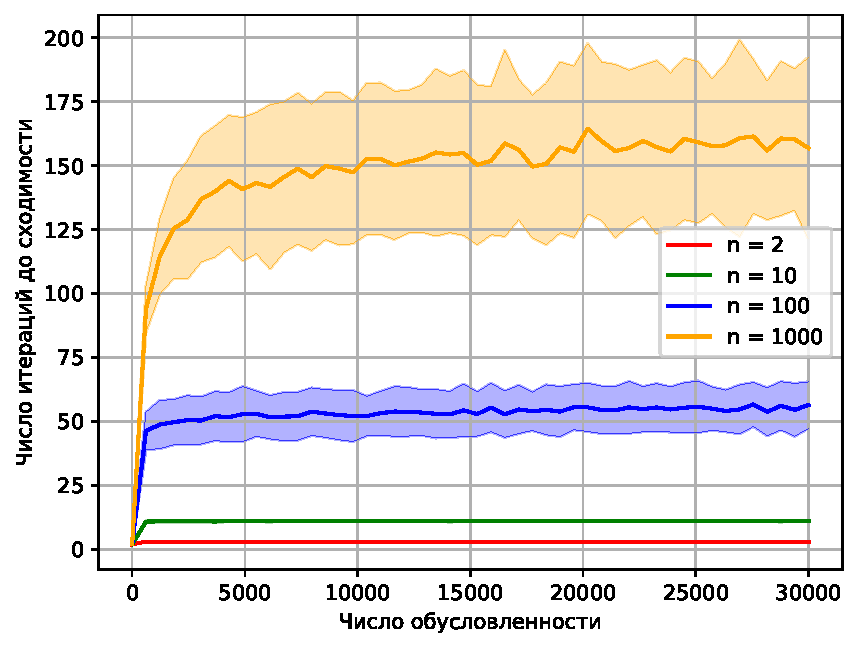
\includegraphics[width=1.0\textwidth]{pics/1/CG_iterations_vs_condition_number.pdf}
\captionsetup{justification=centering}
\caption{Зависимость числа итераций CG от числа обусловленности при разных $n$}
\end{figure}

По всем кривым можно заключить, что число итераций растет с числом обусловленности, как и для градиентного спуска. При этом в отличие от градиентного спуска число итераций прямо пропорционально числу переменных в задаче. CG сходится намного быстрее GD. Более того, со временем число итераций в CG выходит на асимптоту, и это вполне объясняется тем, что метод теоретически должен найти точное решение за $n$ итераций и останавливается раньше по нашему критерию останова. Понятно, что из-за вычислительных погрешностей метод не гарантирует нахождение результата за $n$ итераций, но, тем не менее, похоже, что что число итераций для неточного решения тоже некоторым образом ограничено.



\subsection{Выбор размера истории в методе L-BFGS}

Оценим стоимость итерации L-BFGS. Основная часть вычислительной стоимости находится в функции BFGS\_Multiply. Оценим её сложность: пусть $v, s, y \in \mathbb{R}^n$, тогда
на каждом уровне рекурсии вычисляется 5 скалярных произведений, две операции деления, две операции умножения вектора на скаляр, две операции сложения/вычитания векторов, одно обычное вычитание. То есть: $7n + 2$ мультипликативных операций и $2n + 1$ аддитивная операция, и при этом глубина рекурсии соответствует размеру истории $l$. Из вызова LBFGS\_Direction добавляются $2n + 1$ мультипликативная операция и $2n$ аддитивных. Итого вычисление направления требует $O(nl)$ операций.

Легко видеть, что структура данных $\mathcal{H}$ занимает $O(nl)$ памяти (при этом нужно избегать копирования при рекурсивном вызове, что учтено в коде), так же на каждом уровне рекурсии требуется память для векторов $s, y$ и $v$, которая содержится в стеке одновременно со всех уровней -- итого опять же $O(nl)$. Всего требуется $O(nl)$ памяти.

\

\begin{algorithm}[H]
	\SetAlgoLined
	\SetKwFunction{Mult}{BFGS\_Multiply}
    \SetKwProg{Fn}{function}{}{}
  	
  	\Fn{\Mult{$v$, $\mathcal{H}$, $\gamma_0$}}{
		\If {$\mathcal{H} = \emptyset$}
	  		{\Return{$\gamma_0 v$}}
		$(s, y) \leftarrow$ последняя пара из $\mathcal{H}$ \;
		$\mathcal{H}' \leftarrow H$ без последней пары \;
		$v' \leftarrow v - \frac{\langle s, v \rangle}{\langle y, s \rangle}y$ \;
		$z \leftarrow  BFGS\_Multiply (v', \mathcal{H}', \gamma_0) $ \;
		\Return{$z + \frac{\langle s, v \rangle - \langle y, z \rangle}{\langle y, s \rangle}s$}
  	}
\caption{Рекурсивное умножение L-BFGS матрицы на вектор}

\label{alg:mult}
\end{algorithm}

\

\begin{algorithm}[H]
	\SetAlgoLined
	\SetKwFunction{Dir}{LBFGS\_Direction}
    \SetKwProg{Fn}{function}{}{}
  	
  	\Fn{\Dir{$f$, $x_k$, $\mathcal{H}_k$}}{
  		$(s, y) \leftarrow$ последняя пара из $\mathcal{H}_k$ \;
  		$\gamma_0 \leftarrow \frac{\langle y, s \rangle}{\langle y, y \rangle}$ \;
		\Return{$\text{BFGS\_Multiply}(-\nabla f(x_k)$, $\mathcal{H}_k$, $\gamma_0)$}
  	}
\caption{Вычисление направления поиска $d_k$ в методе L-BFGS}
\label{alg:direction}
\end{algorithm}

\

Взглянем на значения функции потерь логистической регрессии в ходе работы L-BFGS на наборе данных $gisette$ при разных значениях размера истории $l$.
Остальные параметры выбраны по умолчанию: $\varepsilon=10^{-4}$, максимальное число итераций -- $500$, для линейного поиска используется стратегия Вульфа с $c_1=10^{-4}$ и $c_2=0.9$.
\newpage
\begin{figure}[H]
	\captionsetup{font=scriptsize}

	\centering
%	\begin{tabular}[c]{cc}
		\subfloat{
    		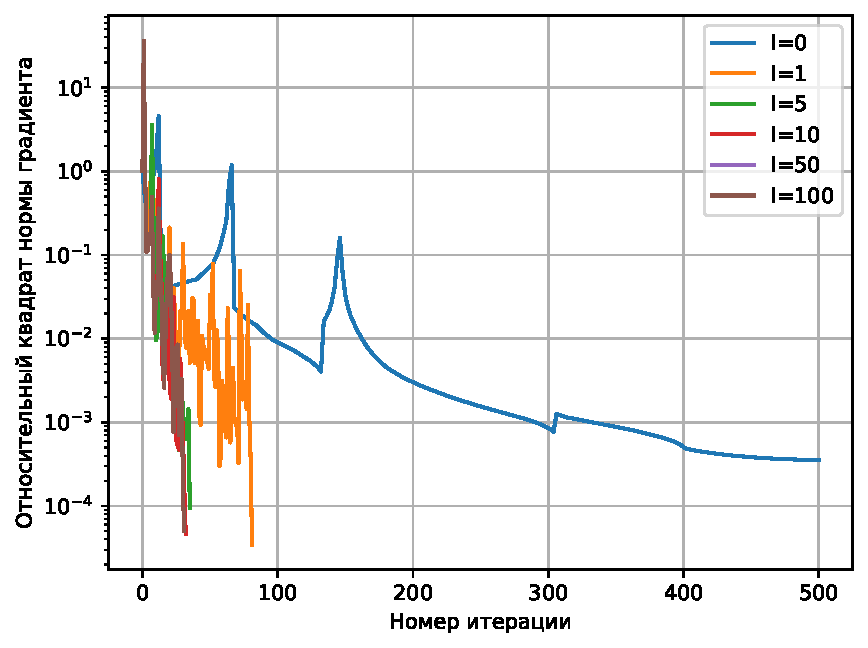
\includegraphics[width=.7\textwidth]{pics/2/lbfgs_grad_norm_vs_iter.pdf}
 		} %&

		\subfloat{
    		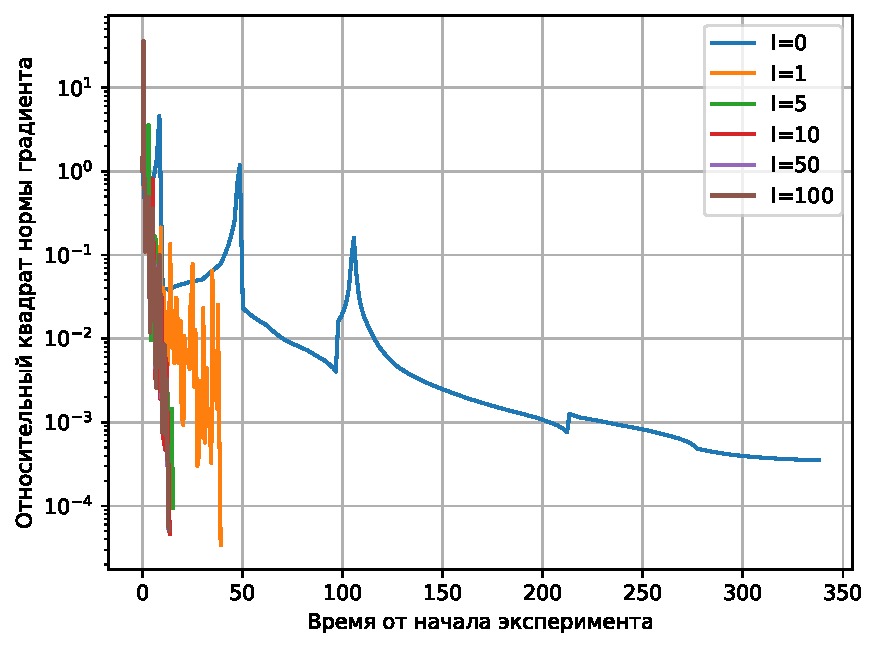
\includegraphics[width=.7\textwidth]{pics/2/lbfgs_grad_norm_vs_time.pdf}
 		}
%   \end{tabular}
   \captionsetup{justification=centering}
   \caption{Графики зависимостей относительного квадрата нормы градиента от номера итерации и времени при использовании разного размера истории в L-BFGS}

\label{fig:gd_strategies_logreg}
\end{figure} 

Как видно, с ростом $l$ алгоритм сходится быстрее, при этом при $l \ge 10$ кривые сливаются, откуда можно сделать вывод, что нет смысла в размере истории большем, чем 10. Уже при $l=5$ мы также имем сравнимую с $l \ge 10$ скорость сходимости. Отсюда можно заключить, что L-BFGS требует помнить довольно небольшой отрезок истории.


\subsection{Сравнение методов на реальной задаче логистической регрессии}


\hspace{1cm} Сравним GD, HFN и L-BFGS на реальных данных. Перед этим
взглянем на число объектов $m$, число признаков $n$ и разреженность матриц в выборках:
\begin{center}
\begin{tabular}{|c|c|c|c|} 
 \hline
 Данные & $m$ & $n$ & Разреженность\\ [0.5ex] 
 \hline\hline
 w8a & 49749 & 300 & 0.9612\\ 
 \hline
 gisette & 6000 & 5000 & 0.0090\\ 
 \hline
 real-sim & 72309 & 20958 & 0.9976\\ 
 \hline
 rcv1.binary & 19996 & 1355191 & 0.9996\\ 
 \hline
 news20.binary & 20242 & 47236 & 0.9984\\ 
 \hline
\end{tabular}
\end{center}

Параметры всех методов -- по умолчанию:
для L-BFGS и HFN $\varepsilon=10^{-4}$, максимальное число итераций -- $500$, размер истории L-BFGS $l=10$;
в градиентном спуске $\varepsilon=10^{-5}$, максимальное число итераций -- $10000$.

Для линейного поиска во всех методах используется стратегия Вульфа с $c_1=10^{-4}$ и $c_2=0.9$.

\begin{figure}[H]
	\captionsetup{font=scriptsize}
	\centering
	\begin{tabular}[c]{cc}
		\subfloat{
    		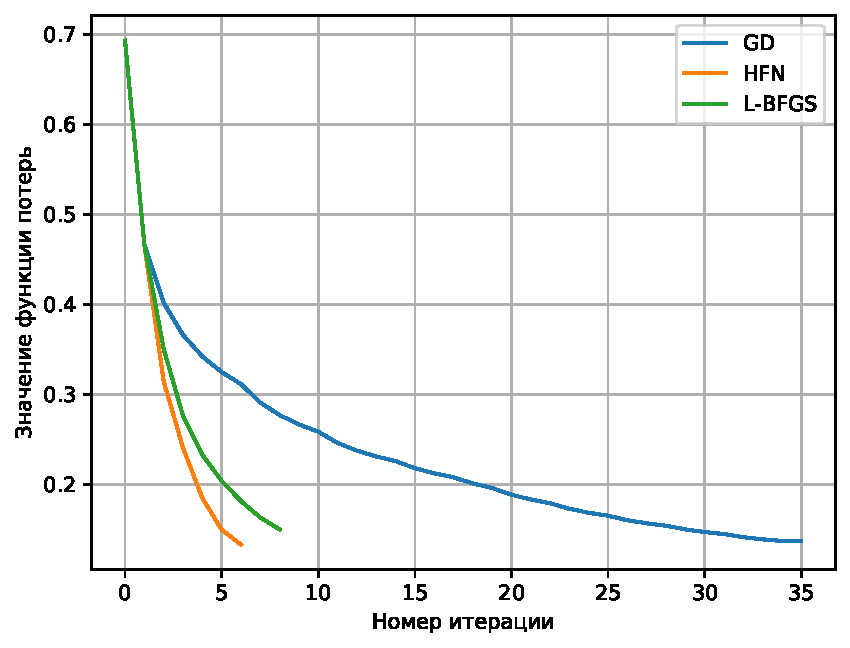
\includegraphics[width=.33\textwidth]{pics/3/logreg_loss_value_vs_iter_w8a.pdf}
 		} &

		\subfloat{
    		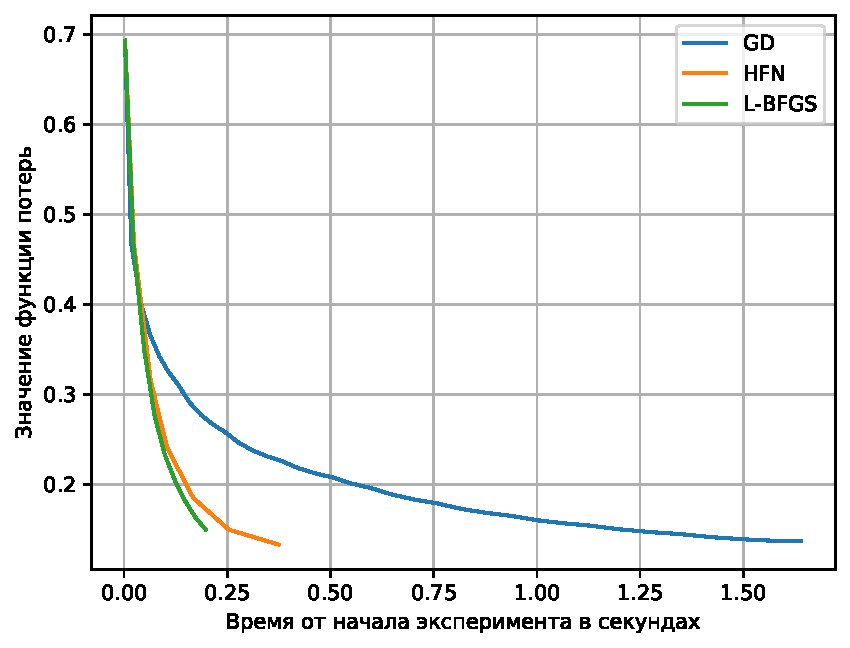
\includegraphics[width=.33\textwidth]{pics/3/logreg_loss_value_vs_time_w8a.pdf}
 		}

		\subfloat{
    		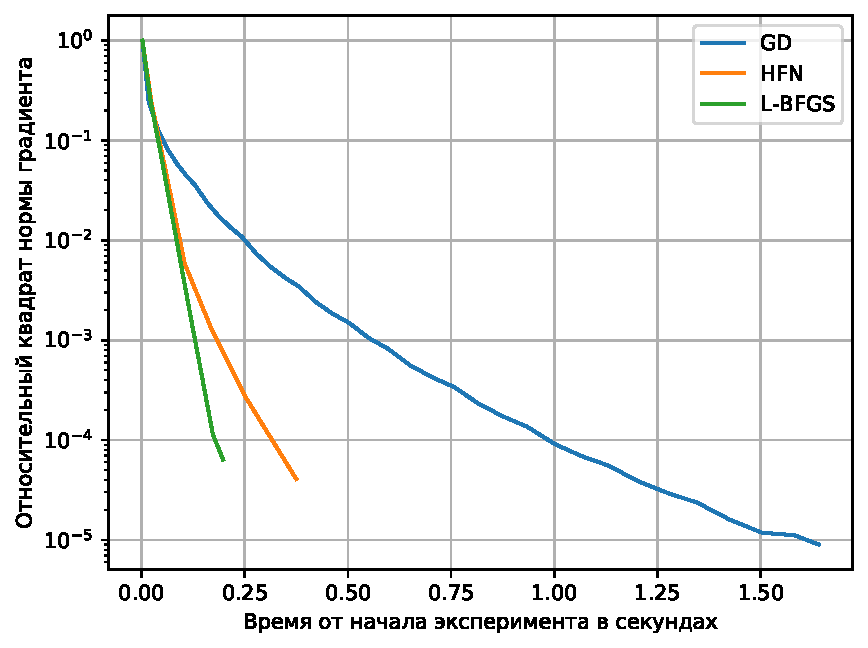
\includegraphics[width=.33\textwidth]{pics/3/logreg_grad_norm_vs_time_w8a.pdf}
 		}

   \end{tabular}
   \captionsetup{justification=centering}
   \caption{Сравнение GD, HFN, L-BFGS на наборе данных $w8a$ \\
   			Число итераций до сходимости: 36, 7, 9;
   			время: 1.640, 0.375, 0.197 секунд \\
   			для GD, HFN и L-BFGS соответственно}
\end{figure}

\begin{figure}[H]
	\captionsetup{font=scriptsize}
	\centering
	\begin{tabular}[c]{ccc}
		\subfloat{
    		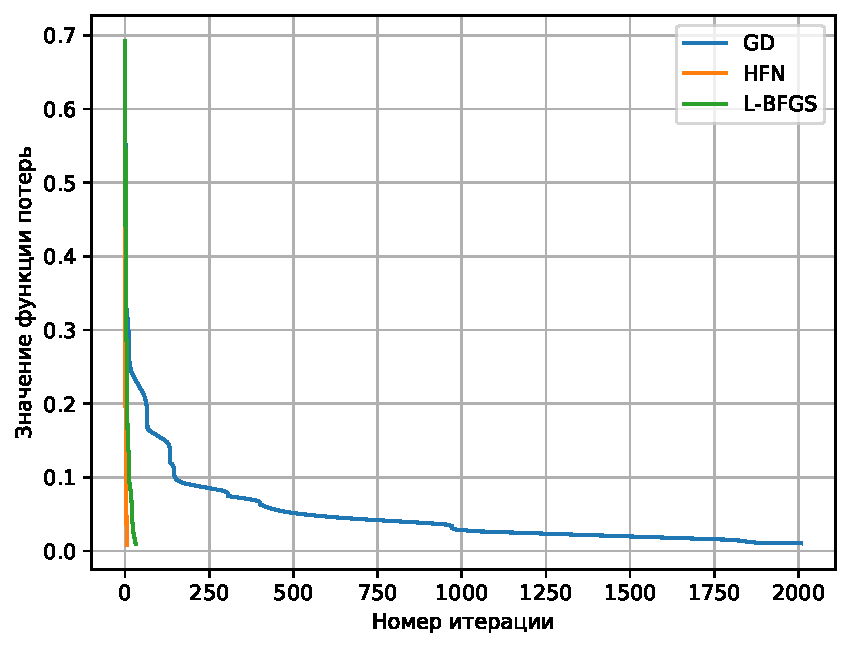
\includegraphics[width=.33\textwidth]{pics/3/logreg_loss_value_vs_iter_gisette_scale.pdf}
 		} &

		\subfloat{
    		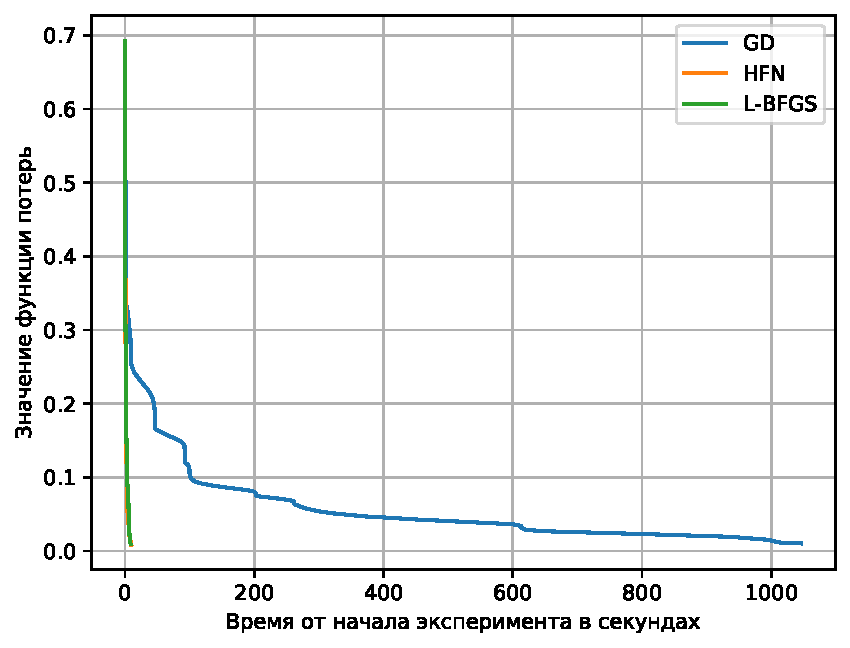
\includegraphics[width=.33\textwidth]{pics/3/logreg_loss_value_vs_time_gisette_scale.pdf}
 		} &
 		
 		\subfloat{
    		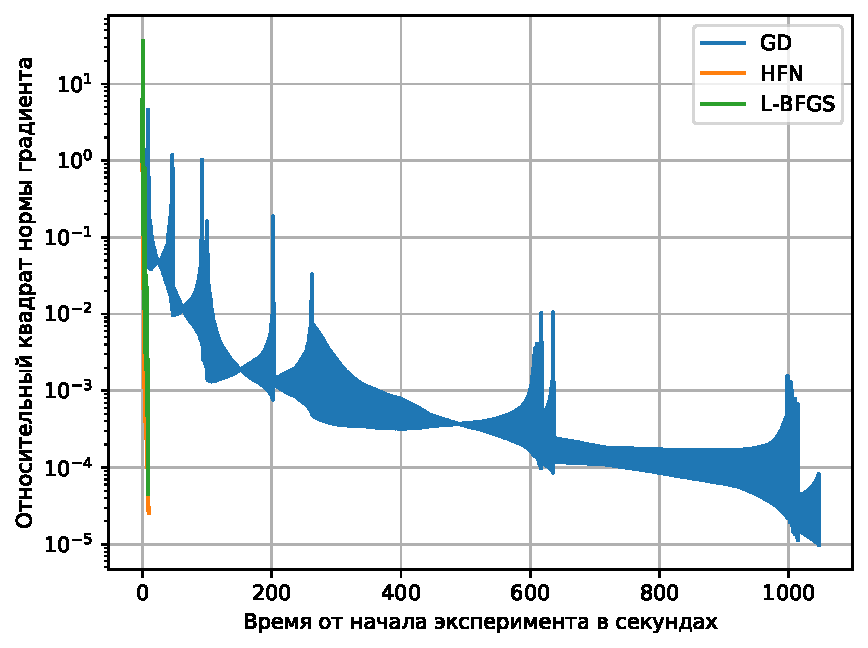
\includegraphics[width=.33\textwidth]{pics/3/logreg_grad_norm_vs_time_gisette_scale.pdf}
 		}
   \end{tabular}
   \captionsetup{justification=centering}
   \caption{Сравнение GD, HFN, L-BFGS на наборе данных $gisette$ \\
   			Число итераций до сходимости: 2010, 7, 33;
   			время: 1046.464, 9.559, 8.652 секунд \\
   			для GD, HFN и L-BFGS соответственно}
\end{figure}


\begin{figure}[H]
	\captionsetup{font=scriptsize}
	\centering
	\begin{tabular}[c]{cc}
		\subfloat{
    		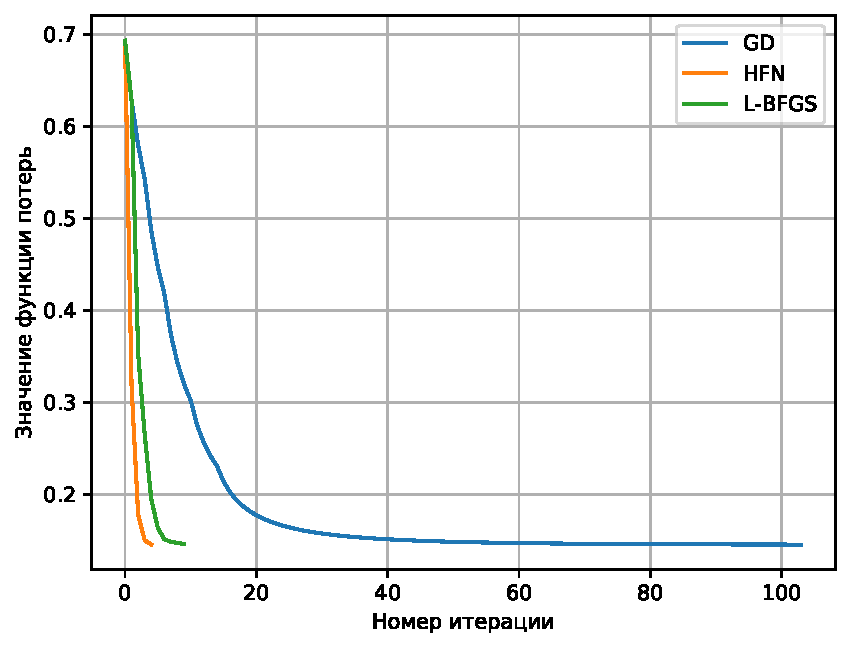
\includegraphics[width=.33\textwidth]{pics/3/logreg_loss_value_vs_iter_real-sim.pdf}
 		} &

		\subfloat{
    		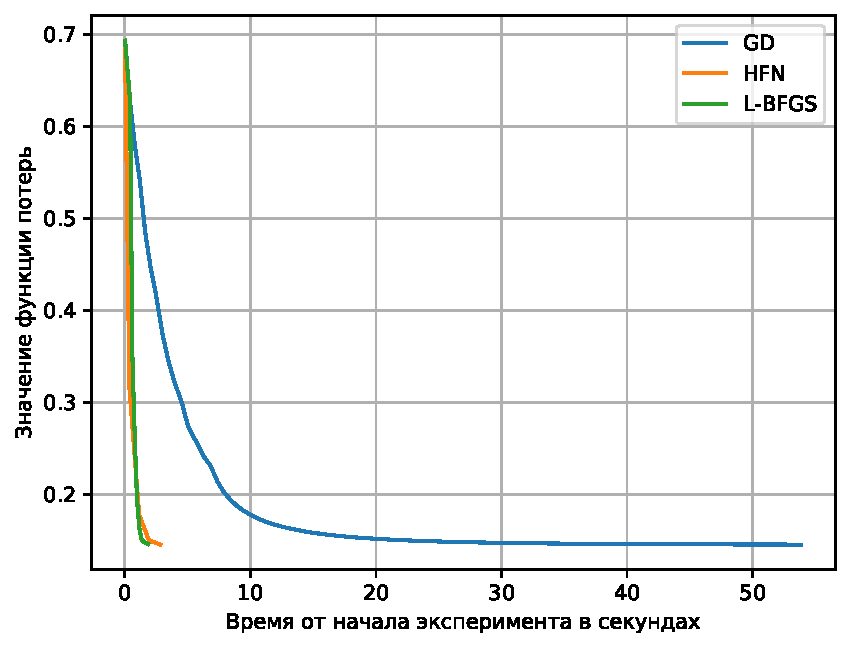
\includegraphics[width=.33\textwidth]{pics/3/logreg_loss_value_vs_time_real-sim.pdf}
 		}

		\subfloat{
    		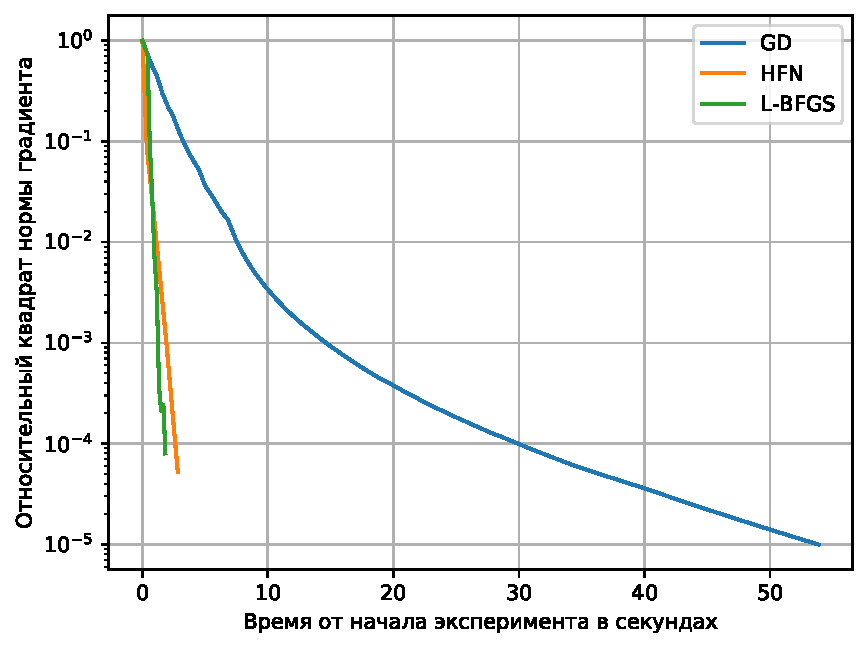
\includegraphics[width=.33\textwidth]{pics/3/logreg_grad_norm_vs_time_real-sim.pdf}
 		}
   \end{tabular}
   \captionsetup{justification=centering}
   \caption{Сравнение GD, HFN, L-BFGS на наборе данных $real$-$sim$ \\
   			Число итераций до сходимости: 104, 5, 10;
   			время: 53.877, 2.834, 1.848 секунд \\
   			для GD, HFN и L-BFGS соответственно}
\end{figure}

\begin{figure}[H]
	\captionsetup{font=scriptsize}
	\centering
	\begin{tabular}[c]{cc}
		\subfloat{
    		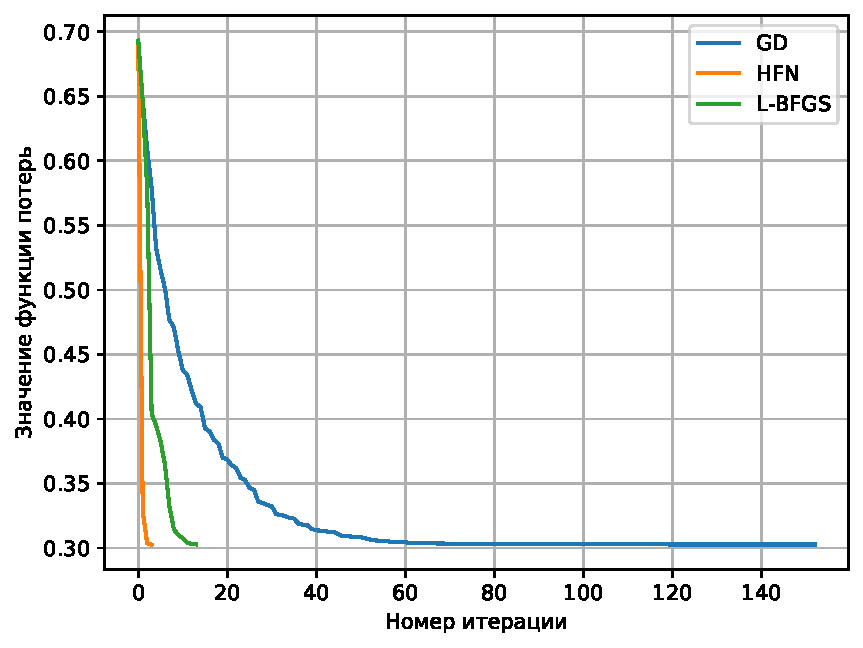
\includegraphics[width=.33\textwidth]{pics/3/logreg_loss_value_vs_iter_news20.pdf}
 		} &

		\subfloat{
    		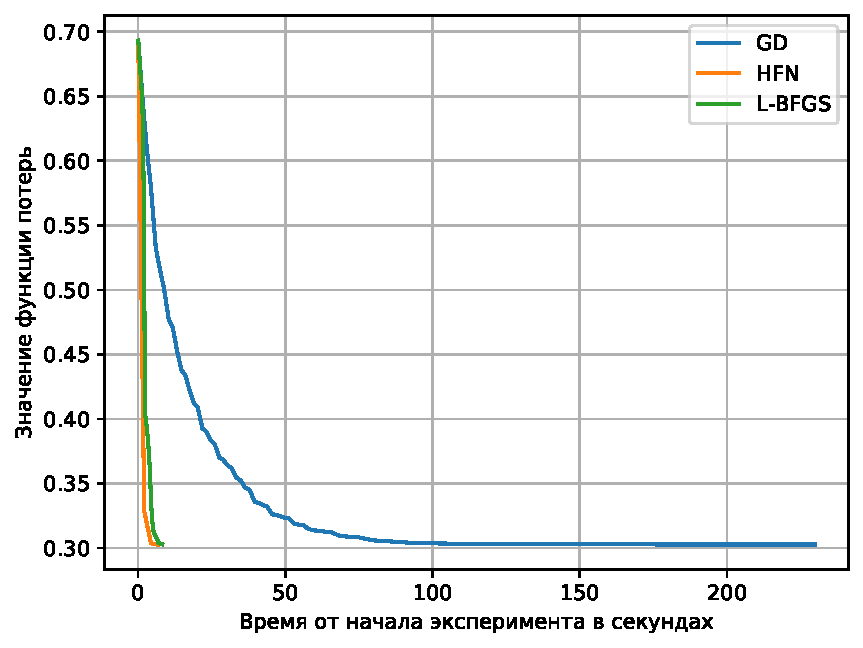
\includegraphics[width=.33\textwidth]{pics/3/logreg_loss_value_vs_time_news20.pdf}
 		}

		\subfloat{
    		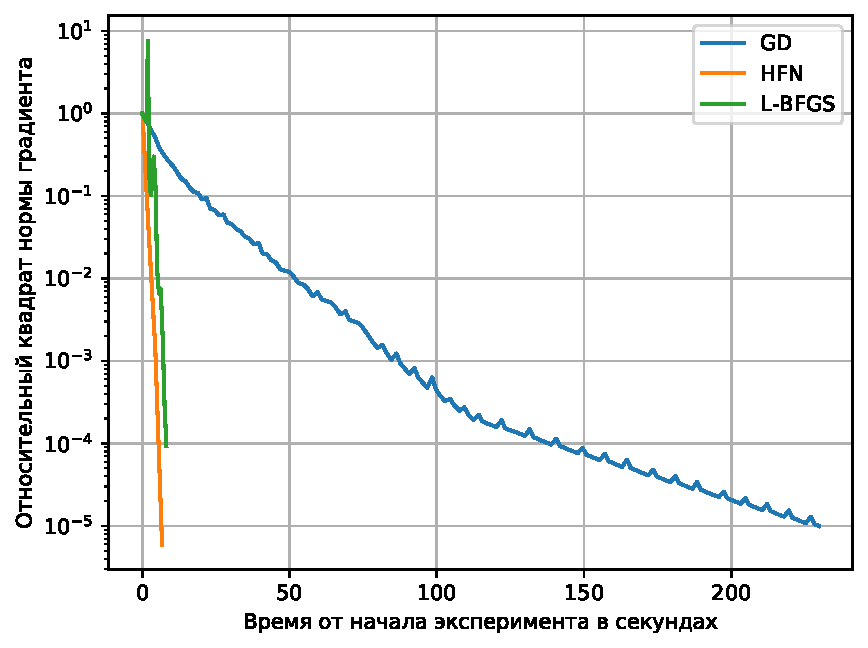
\includegraphics[width=.33\textwidth]{pics/3/logreg_grad_norm_vs_time_news20.pdf}
 		}
  
   \end{tabular}
   \captionsetup{justification=centering}
   \caption{Сравнение GD, HFN, L-BFGS на наборе данных $news20.binary$  \\ 			Число итераций до сходимости: 153, 4, 14;
   			время: 229.747, 6.726, 8.205 секунд \\
   			для GD, HFN и L-BFGS соответственно}
\end{figure}

\begin{figure}[H]
	\captionsetup{font=scriptsize}
	\centering
	\begin{tabular}[c]{cc}
		\subfloat{
    		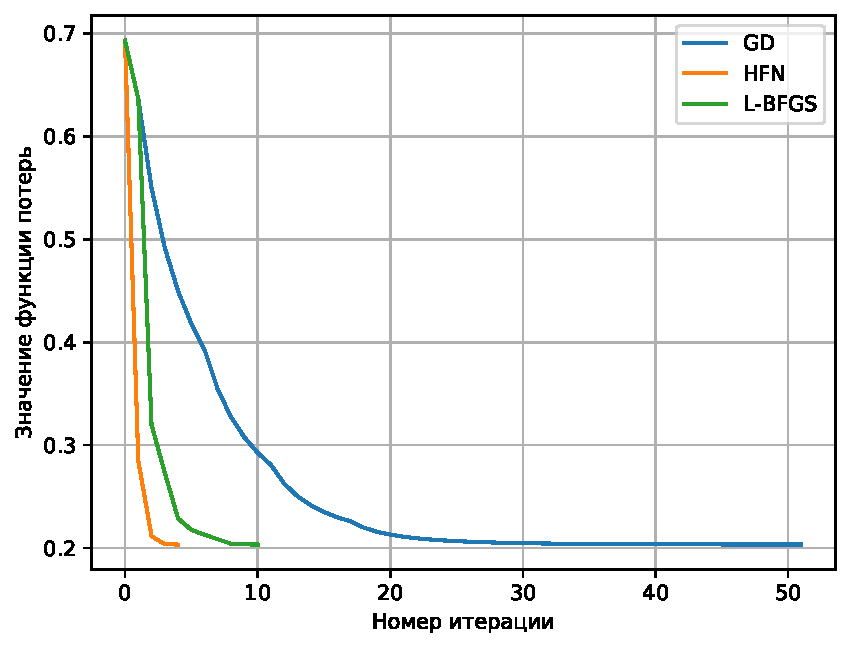
\includegraphics[width=.33\textwidth]{pics/3/logreg_loss_value_vs_iter_rcv1_train.pdf}
 		} &

		\subfloat{
    		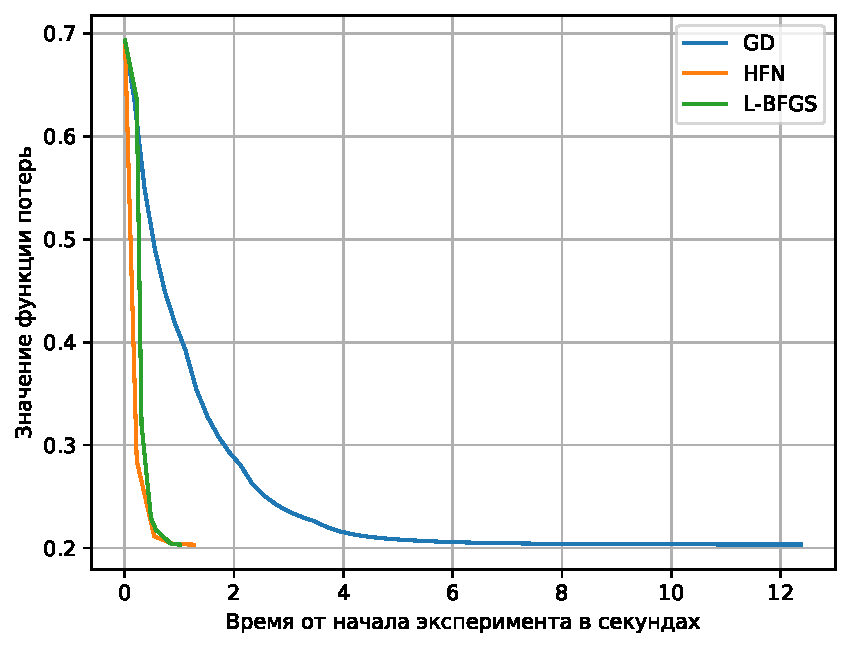
\includegraphics[width=.33\textwidth]{pics/3/logreg_loss_value_vs_time_rcv1_train.pdf}
 		}

		\subfloat{
    		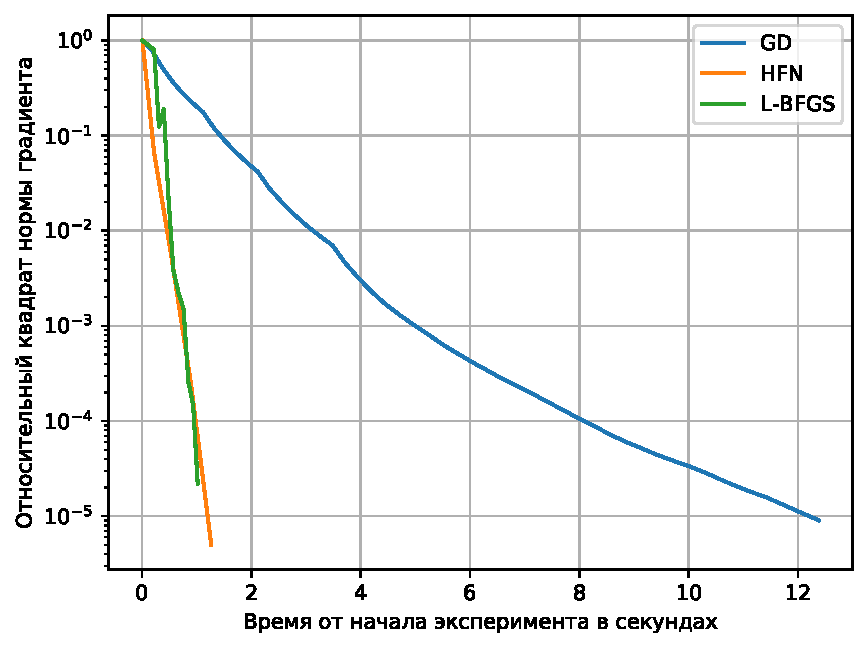
\includegraphics[width=.33\textwidth]{pics/3/logreg_grad_norm_vs_time_rcv1_train.pdf}
 		}
   \end{tabular}
   \captionsetup{justification=centering}
   \caption{Сравнение GD, HFN, L-BFGS на наборе данных $rcv1.binary$ \\
   			Число итераций до сходимости: 52, 5, 11;
   			время: 12.378, 1.267, 1.021 секунд \\
   			для GD, HFN и L-BFGS соответственно}
\end{figure}

В первую очередь мы наблюдаем на графиках превосходство HFN и L-BFGS над GD во всех случаях. L-BFGS сходится к оптимуму за большее число итераций, чем HFN, но быстрее по времени в 4 из 5 случаев. Стоит заметить, что число итераций HFN на $gisette$ совпадает с числом итераций метода Ньютона в прошлом практическом задании, но метод Ньютона тогда потребовал для сходимости 50 минут. HFN же справился за 9 с половиной секунд.

\section{Выводы.}
Мы изучили поведение методов и увидели их преимущества в сравнении с градиентным спуском, увидели, что методы HFN и L-BFGS достигают скорости сходимости по времени, недостижимой градиентным спуском, сохраняют достоинства метода Ньютона, имея сильно меньшую стоимость итерации. Также мы пронаблюдали работу L-BFGS в зависимости от размера истории и пришли к выводу, что для быстрой сходимости метода достаточно лишь небольшой истории с предыдущих итераций.
\end{document}